\section{Notions théoriques}

\paragraph{Docker} Docker est une plateforme open-source qui permet de créer, de déployer et de gérer des applications
de manière isolée, dans des conteneurs légers. Son objectif principal est de faciliter la mise en œuvre et
la gestion des environnements de développement, des tests et des déploiements d'applications. En
utilisant Docker, il est possible de créer des conteneurs contenant tous les éléments nécessaires à
l'exécution d'une application, y compris les dépendances et les configurations, et de les exécuter de
manière cohérente sur différentes machines.

\paragraph{Replica sets} Un replica set est un mécanisme de réplication dans MongoDB qui permet de maintenir plusieurs copies
identiques des données sur différents serveurs. L'objectif principal des replica sets est d'améliorer la
disponibilité et la tolérance aux pannes d'une base de données. Chaque replica set comprend un nœud
principal (primary node) qui accepte les opérations d'écriture et plusieurs nœuds secondaires
(secondary nodes) qui répliquent les données du nœud principal. En cas de défaillance du nœud
principal, l'un des nœuds secondaires peut être élu comme nouveau nœud principal, assurant ainsi la
continuité du service. Les replica sets offrent également une répartition de charge en redirigeant les
opérations de lecture vers les nœuds secondaires

\paragraph{Sharding} Le sharding est une technique utilisée dans les bases de données pour distribuer les données sur
plusieurs serveurs, appelés des shards, afin de répartir la charge et d'améliorer les performances.
Lorsqu'une base de données devient trop volumineuse pour être gérée par un seul serveur, le sharding
permet de diviser les données en fragments (shards) et de les stocker sur plusieurs serveurs. Chaque
shard contient une partie des données et peut être consulté indépendamment des autres. Cela permet
d'augmenter la capacité de stockage et de traitement des données, ainsi que de paralléliser les
requêtes.

En combinant Docker, le sharding et les replica sets, il est possible de déployer et de gérer des bases de
données distribuées, résilientes et hautement disponibles. Docker permet de créer des conteneurs
isolés pour exécuter les instances de base de données, tandis que le sharding et les replica sets assurent
la répartition des données et la redondance des serveurs pour améliorer les performances et la fiabilité
du système.

\section{Partie pratique}

J'ai d'abord créé tout dans un docker à l'aide de docker-compose.
Ceci était plus simple car comme ça cela créé tout en même temps et on n'a plus qu'a les initialiser
après

On a donc créé 3 types : Shard, Mongos et config Servers:

\begin{itemize}
    \item Le shard : Il contiendra donc une partie des données, chaque shard peuvent être déployé en
    tant que replica sets
    \item Mongos : Il va agir comme « routeur » il fournira donc une interface à chaque client de
    l'application
    \item Config servers : C'est là où on va enregistrer les configurations pour le cluster
\end{itemize}

On va donc d'abord créer 3 serveurs de sharding et ensuite créer donc ces replica sets.
Les avantages à ceux-ci sont nombreux :

\begin{itemize}
    \item \textbf{Haute disponibilité} : On assure donc la redondance des données pour la gestion du sharding. Si
    un des membres tombent en panne cela assure toujours la mise en place de ce sharding
    \item \textbf{Optimisation des ressources }: En configurant le sharding avant les replica sets, vous pouvez
    évaluer la charge de travail et les besoins de chaque shard individuellement avant de déployer
    des replica sets. Cela vous permet d'optimiser l'allocation des ressources en fonction des
    exigences spécifiques de chaque shard, plutôt que de provisionner des replica sets pour tous les
    shards dès le départ.
    \item \textbf{Flexibilité dans l'ajout de replica sets }: En configurant d'abord le sharding, vous pouvez ajouter
    des replica sets à chaque shard au fur et à mesure de vos besoins. Cela vous offre une plus
    grande flexibilité dans l'ajustement de la capacité de stockage et de traitement de chaque shard
    individuellement, en ajoutant des membres supplémentaires aux replica sets existants ou en
    créant de nouveaux replica sets si nécessaire.
    \item \textbf{Évolutivité}: Le sharding permet de répartir les données sur plusieurs shards, ce qui permet
    d'atteindre une capacité de stockage et une capacité de traitement beaucoup plus importantes.
    L'utilisation de replica sets avec sharding permet de répartir également la charge de travail sur
    les membres du replica set, offrant ainsi une meilleure évolutivité horizontale de l'ensemble du
    système.
    \item \textbf{Simplification de la configuration initiale }: En configurant d'abord le sharding, vous pouvez
    réduire la complexité de la configuration initiale, en vous concentrant d'abord sur la mise en
    place de la répartition des données sur plusieurs shards. Une fois que le sharding est en place et
    que vous avez évalué les performances, vous pouvez ensuite configurer les replica sets pour
    chaque shard individuellement.
\end{itemize}

\begin{figure}[H]
    \centering
    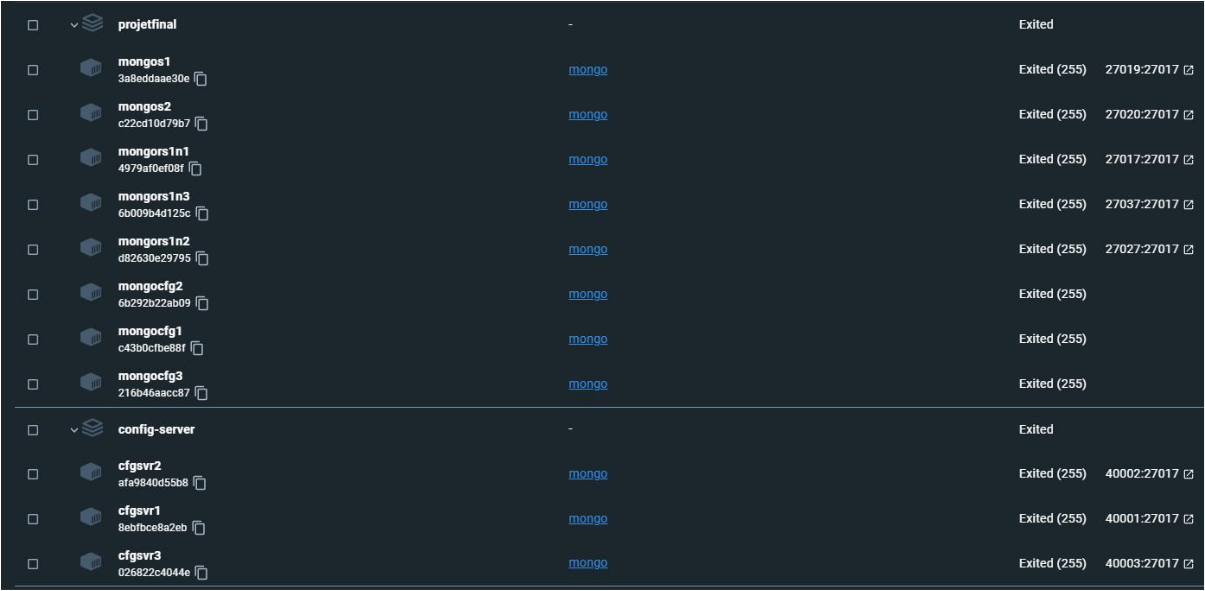
\includegraphics[width=\textwidth]{./img/alex.png}
    \caption{Instances des containeurs de MongoDB}
    \label{fig:alex-container-instance}
\end{figure}

On peut donc voir les différents type d'instance docker créé pour chacun des shardings, routeurs, config
servers.

Voici un aperçu de la structure de notre docker-compose (voir sur github) :
Nous définissons trois noeuds de shard (mongorsn1, mongors1n2, mongors1n3) en utilisant l'image
Docker "mongo". Chaque noeud est configuré en tant que shard avec le paramètre "--shardsvr". Ils
appartiennent tous au même replica set "mongors1" et utilisent le dossier "/data/db" pour stocker les
données. Chaque noeud est exposé sur le port 27017 à la fois dans le conteneur et sur la machine hôte.

Nous définissons trois noeuds de configuration (mongocfg1, mongocfg2, mongocfg3) également en
utilisant l'image Docker "mongo". Ces noeuds sont configurés en tant que serveurs de configuration
avec le paramètre "--configsvr". Ils appartiennent tous au même replica set de configuration
"mongors1conf" et utilisent le dossier "/data/db" pour stocker les données de configuration. Chaque
noeud de configuration est exposé sur le port 27017 à la fois dans le conteneur et sur la machine hôte.

Nous définissons deux noeuds de mongos (mongos1, mongos2) en utilisant l'image Docker "mongo".
Ces noeuds sont responsables du routage des requêtes vers les shards. Chaque noeud de mongos
dépend des noeuds de configuration (mongocfg1, mongocfg2) pour obtenir les informations de
configuration. Les noeuds mongos sont exposés sur les ports 27019 et 27020 dans le conteneur et sur
les ports correspondants sur la machine hôte.

Après avoir créé ceci on va donc tous les initialisés j'ai donc utilisés ces différentes commandes (voir sur
github)

\section{Conclusion}

C'était la première fois que je travaillais avec Docker. Donc j'ai dû me familiariser au début pendant
quelques heures. Ensuite la création des Replica sets ainsi que du sharding a été assez complexe. J'ai
d'abord fait tout cela dans docker-compose mais cela ne parvenait pas à fonctionner j'ai donc seulement
laisser les différentes parties déjà créées et pour la création des shardings,... J'ai fait cela directement
par ligne de commande dans chaque BD (ceci est donc expliqué sur github)

Le déroulement du projet s'est bien passé globalement. Le manque de temps a été un défi majeur dans
ce projet. En raison d'un certain nombre d'autres projets en cours, j'ai dû gérer mes priorités et trouver
des moyens d'optimiser mon temps pour accomplir les tâches nécessaires. Cela m'a permis de
développer mes compétences en gestion du temps et en prise de décisions rapides.

En travaillant sur ce projet, j'ai pu constater l'importance de la planification et de la documentation. La
complexité des Replica Sets et du sharding m'a poussé à organiser mes idées, à créer des diagrammes et
à documenter les étapes importantes. Cela s'est avéré bénéfique pour moi-même et pour l'équipe, car
cela nous a permis de suivre plus facilement le processus de développement.
